\documentclass[a4paper]{article}
\usepackage[left=1cm, right=1cm, top=1cm, bottom=1cm]{geometry}
% put the command
%
% \input{odl_preamble.tex}
%
% at the top of your latex file (just after the \documentclass) to include this
% in your document.  Feel free to add to this file, but please consider adding
% commands and packages that are specific to your work outside of this file:
% let's reserve this file for stuff that most of us would need.

% The amssymb package provides various useful mathematical symbols
\usepackage{amsmath}
\usepackage{amsfonts}
\usepackage{amssymb}
\usepackage{amsthm}
\usepackage{graphicx} % for includegraphics
\usepackage{xspace} % needed for \eg, \ie, \etc
\usepackage{bm} % for bold math
%\usepackage{threeparttable} % for tables with footnotes
\usepackage{subcaption}
\usepackage{caption}
\usepackage{graphicx}
\usepackage{fullpage}
\usepackage{textcomp}
\usepackage{listings}
\usepackage{xcolor}
\usepackage{float}
\usepackage{stmaryrd}
\usepackage[toc,page]{appendix}

\usepackage[ruled,lined,linesnumbered]{algorithm2e}

% hyperref must be last
\usepackage{hyperref}
\hypersetup{
  colorlinks=true,
  linkcolor=red,
  citecolor=green,
  urlcolor=blue
}
  
% We often use mathcal for functions
\newcommand{\fnc}[1]{\ensuremath{\mathcal{#1}}}
\newcommand{\vecfnc}[1]{\ensuremath{\boldsymbol{\mathcal{#1}}}} % vector function

% matrices are often math sans serif type
\newcommand{\mat}[1]{\ensuremath{\mathsf{#1}}}

\newcommand{\Pm}[0]{\psi_h^{(n-1)}}
\newcommand{\Pn}[0]{\psi_h^{(n)}}
\newcommand{\Pnn}[0]{\psi_h^{(n+1)}}
\newcommand{\Qn}[0]{q_h^{(n)}}
\newcommand{\Qnn}[0]{q_h^{(n+1)}}

\newcommand{\Sn}[0]{s_h^{(n)}}
\newcommand{\Snn}[0]{s_h^{(n+1)}}
\newcommand{\Lht}[0]{L_{h,\Delta t}}

% SBP operator matrices
\newcommand{\M}[0]{\mat{M}}
\newcommand{\Dx}[0]{\mat{D}_{x}}
\newcommand{\Dy}[0]{\mat{D}_{y}}
\newcommand{\Dz}[0]{\mat{D}_{z}}
\newcommand{\Sx}[0]{\mat{S}_{x}}
\newcommand{\Sy}[0]{\mat{S}_{y}}
\newcommand{\Sz}[0]{\mat{S}_{z}}
\newcommand{\Qx}[0]{\mat{Q}_{x}}
\newcommand{\Qy}[0]{\mat{Q}_{y}}
\newcommand{\Qz}[0]{\mat{Q}_{z}}
\newcommand{\Ex}[0]{\mat{E}_{x}}
\newcommand{\Ey}[0]{\mat{E}_{y}}
\newcommand{\Ez}[0]{\mat{E}_{z}}
\newcommand{\Par}[2]{\frac{\partial {#1}}{\partial{#2}}}
% optimization commands
\newcommand{\Lag}[0]{\fnc{L}}
\newcommand{\optmin}{\ensuremath{\text{minimize}}}
\newcommand{\wrt}{\ensuremath{\text{with respect to}}}
\newcommand{\st}[0]{\ensuremath{\text{s.t.}}}
\newcommand{\W}[0]{\mat{W}} % Hessian
\newcommand{\A}[0]{\mat{A}} % Jacobian
\newcommand{\K}[0]{\mat{K}} % KKT matrix
\newcommand{\Hess}[0]{\mat{H}} % upper Hessenberg
\newcommand{\I}[0]{\mat{I}} % identity
\newcommand{\diff}[0]{\mathrm{d}}
% common math operators
\DeclareMathOperator{\spn}{span}
\DeclareMathOperator{\range}{range}
\DeclareMathOperator{\mydiag}{diag}
\newcommand{\argmin}[0]{\ensuremath{\operatornamewithlimits{argmin}}}
\newcommand{\sgn}[0]{\operatorname{sgn}}
\newcommand{\nullsp}[0]{\operatorname{null}}

% environments for definitions, therorems, etc 
\newtheorem{definition}{Definition}
\newtheorem{proposition}{Proposition}
\newtheorem{corollary}{Corollary}
\newtheorem{lemma}{Lemma}
\newtheorem{remark}{Remark}
\newtheorem{assumption}{Assumption}
\newtheorem{thrm}{Theorem}

% command latin phrases and other short-forms
\newcommand{\etal}[0]{{\em et~al.\@}\xspace}
\newcommand{\eg}[0]{{e.g.\@}\xspace}
\newcommand{\ie}[0]{{i.e.\@}\xspace}
\newcommand{\viz}[0]{{viz.\@}\xspace}
\newcommand{\resp}[0]{{resp.\@}\xspace}

\newcommand{\Jump}[1]{\llbracket #1\rrbracket}
\newcommand{\Mean}[1]{\{\{#1\}\}}
% Misc. commands
\newcommand{\ignore}[1]{} % comment out large sections of code


\title{Assignment 1: Adjoint of Elliptic Equation}
\author{ID:4873}
\begin{document}
 \maketitle
 
\begin{abstract}
   Given a general elliptic equation with spatially varying diffusion coefficient, we derived the corresponding continuous adjoint equation. A symmetric interior penalty discontinuous (SIPG) Galerkin method which is implemented, as well as the discrete adjoint. The primal solution accuracy is verified through methods of manufactured solution. Furthermore, the discrete adjoint equation is also solved to verify the adjoint consistency. The results show that both the primal solution and adjoint solution achieve the design accuracy, and that the adjoint solution is smooth when the adjoint problem is well-posed. 
\end{abstract}

\section{Continuous adjoint equation} \label{sec:con_adj}
The primal elliptic PDE is defined as
\begin{equation} \label{eq:primal_pde}
\begin{aligned}
-\nabla\cdot (\gamma\nabla u) &= f,	\quad && \forall(x,y)\in\Omega, \\
u(x,y) &= u_{\partial\Omega}(x,y), \quad&&\forall(x,y)\in\partial\Omega,
\end{aligned}
\end{equation}
and the functional is 
\begin{equation}\label{eq:functional}
\begin{aligned}
\mathcal{J}=\int_{\partial\Omega_{1}}\beta\gamma(\vec{n}\cdot\nabla u) \diff \Gamma
\end{aligned}
\end{equation}

The continuous adjoint equation can be derived as follows:

\begin{equation}
\begin{aligned}
	\fnc{J} &= \int_{\partial\Omega_{1}}\beta\gamma(\vec{n}\cdot\nabla u) \diff x \\
	&=\int_{\partial\Omega_{1}}\beta\gamma(\vec{n}\cdot\nabla u) \diff\Gamma + \int_{\Omega} \psi(-\nabla\cdot (\gamma\nabla u) - f)\diff\Omega \\
	&=\int_{\partial\Omega_{1}}\beta\gamma(\vec{n}\cdot\nabla u) \diff\Gamma - \int_{\partial\Omega} \psi\gamma\vec{n}\cdot\nabla u\diff\Gamma + \int_{\Omega} \gamma\nabla\psi\cdot \nabla u\diff\Omega - \int_{\Omega}\psi f\diff\Omega \\
	&=\int_{\partial\Omega_{1}}\beta\gamma(\vec{n}\cdot\nabla u) \diff\Gamma - \int_{\partial\Omega} \psi\gamma\vec{n}\cdot\nabla u\diff\Gamma + \int_{\partial\Omega}\gamma u\vec{n}\cdot\nabla\psi\diff\Gamma  - \int_{\Omega} u\nabla\cdot(\gamma  \nabla \psi)\diff\Omega - \int_{\Omega}\psi f\diff\Omega \\
	&= \int_{\partial\Omega_{1}}(\beta - \psi)\gamma(\vec{n}\cdot\nabla u) \diff\Gamma - \int_{\partial\Omega\backslash\partial\Omega_{1}}\psi\gamma(\vec{n}\cdot\nabla u) \diff\Gamma + \int_{\partial\Omega}\gamma u_{\partial\Omega}\vec{n}\cdot\nabla\psi\diff\Gamma - \int_{\Omega} u\nabla\cdot (\gamma \nabla \psi)\diff\Omega - \int_{\Omega}\psi f\diff\Omega \\
\end{aligned}
\end{equation}
Note we used integration by parts twice in the above derivation. The duality requires that primal solution $u$ can be eliminate from the functional, which can be satisfied if
\begin{equation} \label{eqn:con_adj}
\begin{aligned}
	-\nabla\cdot(\gamma\nabla u) &= 0, \quad \forall (x,y) \in\Omega, \\
	\psi(x,y)  &= \beta, \quad\forall(x,y) \in\partial\Omega_1 \\
	\psi(x,y)  &= 0, \quad\forall(x,y) \in\partial\Omega\backslash\partial\Omega_1 \\
\end{aligned}
\end{equation}

(\ref{eqn:con_adj}) is the continuous adjoint PDE. With it, the functional can be evaluated as
\begin{equation}
	\fnc{J} = \int_{\partial\Omega}\gamma u_{\partial\Omega}\vec{n}\cdot\nabla\psi\diff\Gamma - \int_{\Omega}\psi f\diff\Omega \\
\end{equation}

\section{Discretization of primal PDE and functional}
We use a discontinuous Galerkin finite element method to discretize~\eqref{eq:primal_pde}: the symmetric interior penalty Galerkin (SIPG)~\cite{Shahbazi2005}. We begin by introducing some notations. Let
$\fnc{T}_h$ be a shape-regular subdivision of $\hat{\Omega}$ into disjoint elements $K \in \fnc{T}_h$, and let $\fnc{V}_h$ be a broken function space on $\fnc{T}_h$ such that $\fnc{V}_h(K) \subset H^2$. Furthermore, we denote by $e$ the interior face between $K^+$ and $K^-$, that is, $e=K^+ \cup K^-$, and let $\Gamma_I$ and $\Gamma$ be the set of interior faces and boundary faces, respectively. Additionally, we introduce the standard jump and mean operators on both scalar and vector variables. For interior face $e\in \Gamma_{I}$, these operators are given by
\begin{equation}
\begin{aligned}
\{\{u\}\} = (u^+ + u^-)/2,   \qquad& \{\{\bm{q}\}\} = (\bm{q}^+ + \bm{q}^-)/2, \\
\llbracket u \rrbracket = u^+\bm{n}^+ - u^-\bm{n}^-, \qquad & \llbracket \bm{q}\rrbracket = \bm{q}^+\cdot \bm{n}^+ - \bm{q}^-\cdot\bm{n}^-,
\end{aligned}
\end{equation}
where $\bm{n}^+$ and $\bm{n}^-$ denote the outward unit normals of $\partial K^+$ and $\partial K^-$, respectively, and $u^+$ and $u^-$ are the traces on $e$ from the interior of $K^+$ and $K^-$, respectively. Finally, the subscript $h$ will be used to indicate a function from a finite dimensional space; for example, the approximate solution to the PDE is denoted as $u_h$.
Then the bilinear weak form of~\eqref{eq:primal_pde} reads
\begin{equation}\label{eq:disc_primal_pde}
\begin{aligned}
\hat{R}_h(u_h, v_h) =& \int_{\hat{\Omega}} (-\nabla v_h\cdot \gamma\nabla u_h + f_hv_h)\diff \Omega
+ \int_{\Gamma_{I}}\Jump{v_h}\cdot\Mean{\gamma\nabla u_h}  \diff\Gamma \\
+& \int_{\Gamma_{I}} \Mean{\gamma\nabla v_h}\cdot \Jump{u_h} \diff\Gamma - \int_{\Gamma_{I}} \epsilon \Mean{\gamma}\Jump{u_h}\cdot\Jump{v_h} \diff\Gamma  + \int_{\Gamma} v_h \gamma\nabla u_h\cdot \bm{n} u_h\diff\Gamma \\
+& \int_{\Gamma} (\gamma\nabla v_h)\cdot (u_h-u_D)\diff\Gamma - \int_{\Gamma}\epsilon \gamma (u_h - u_D) \diff\Gamma  \\
=& 0,
\end{aligned}
\end{equation}
where $s_h, v_h,\:u_h\in \fnc{V}_h$ are the discrete body force, the test function and the approximate solution, respectively, $\hat{F}$ is the upwinding flux function, and $\epsilon$ is the SIPG penalty parameter~\cite{Shahbazi2005}:
\begin{equation}\label{eq:disc_func}
\begin{aligned}
\epsilon = 
\begin{cases}
\frac{(p+1)(p+d)}{2d} \frac{ \int_{\Gamma}\diff\Gamma }{ \min (\int_{K^+}\diff\Omega, \int_{K^-}\diff\Omega) }\qquad &on\: \Gamma_I  \\
\frac{(p+1)(p+d)}{d} \frac{ \int_{\Gamma}\diff\Gamma }{ \int_{K}\diff\Omega }\qquad &on\: \Gamma
\end{cases},
\end{aligned}
\end{equation}
where $d$ is the spatial dimension.

According to~\cite{Hartmann2007}, in order to achieve adjoint consistency, we need the so-called interior penalty modification when discretizing the functional:
\begin{equation}
J_h = \int_{\partial\Omega_{1}}\beta\gamma(\vec{n}\cdot\nabla u_h) \diff \Gamma - \int_{\partial\Omega_1}\epsilon \gamma (u_h - u_D) \diff\Gamma 
\end{equation}


\section{Numerical results}
To estimate the asymptotic convergence rate, we use a sequence of uniformly refined meshes consisting of $K=$ 200, 800, 1800, 3200 and 5000 triangular elements. These mesh are obtained by subdividing quadrilaterals in an structured mesh. Furthermore, $p=1,2,3,4$ approximations with Lagrangian basis are used. Both primal and discrete adjoint equation are solved, and the results are summarized as follows:
\begin{itemize}
	\item Figure~\ref{fig:soln_accuracy} plots the $L^2$ errors of the solution versus the mesh size, $h = 2/\sqrt{2K}$. We can see that all the discretizations approximately achieve design accuracy, $p+1$.
	\item Figure~\ref{fig:func_ill} and \ref{fig:func_well} plot the functional error with $\beta=1$ and $\beta=\frac{\pi^2(e^2-1)(e-e^x)}{(e-1)^2}$, respectively. The convergence rates of the former are approximately $p+1$ while the convergence rates for the latter are around $2p$. 
	\item The contours of the adjoint solution are shown in Figure~\ref{fig:adj_contours}. When $\beta=1$, the contours are clustered at the lower left and lower right corners; when $\beta=\frac{\pi^2(e^2-1)(e-e^x)}{(e-1)^2}$ the contours look quite smooth.
	\item The Figure~\ref{fig:convergence} and Figure~\ref{fig:adj_contours} together suggest that with $\beta=1$ (\ref{eq:disc_primal_pde}) and (\ref{eq:disc_func} )are not adjoint consistent, while with $\beta=\frac{\pi^2(e^2-1)(e-e^x)}{(e-1)^2}$ they are.
\end{itemize}

When $\beta=1$, the adjoint equation is ill-posed since at points $(x,y)=(0,0), (1,0)$, the two singular points in Figure~\ref*{fig:adjsln_beta1}, the adjoint solution is double defined. On the other hand, with $\beta=\frac{\pi^2(e^x-1)(e-e^x)}{(e-1)^2}$, the adjoint problem is well-posed (probably also smooth). That is, $\beta=1$ leads to adjoint inconsistency. Actually, the ill-posedness and well-posedness can be verified by either the convergence rate of the corresponding functional or the adjoint solution contour. Specifically, if the adjoint condition is well-posed and smooth ($C^{2p}$), then we can observe an accuracy of $2p$ in the functional for second-order PDEs\cite{Hicken2011} and smooth adjoint solution. On the contrary, if the adjoint solution is either ill-posed or nonsmooth, then we may not see the superconvergence in functional and smoothness in adjoint solution contour. 




%\subsection{Convergence study of primal solution}
%\begin{figure}[!htbp]
%  \centering
%  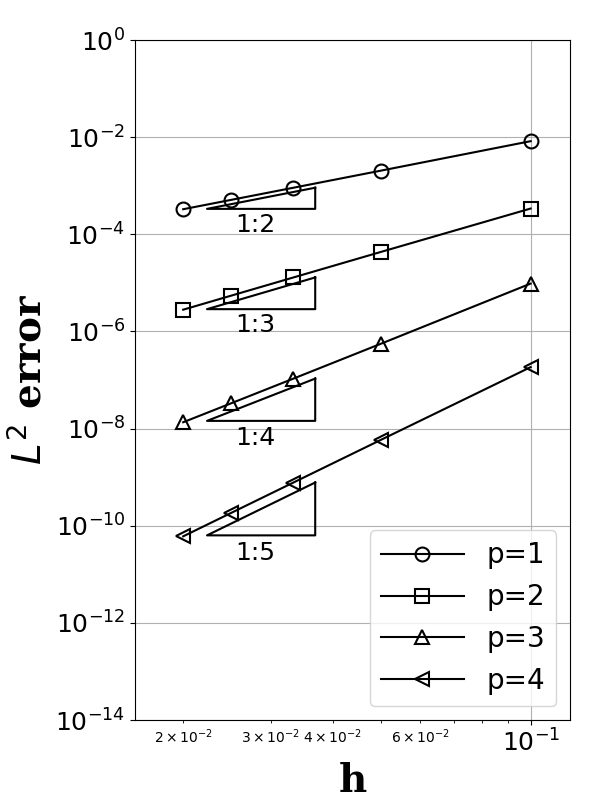
\includegraphics[width=0.45\linewidth]{figures/primal_soln_accuracy.png}
%  \caption{$L^2$ error of primal solution}
%  \label{fig:soln_accuracy1}
%\end{figure}
\subsection{Convergence study of adjoint solution}
\begin{figure}[!htbp]
  \centering
  \begin{subfigure}{0.325\textwidth}
    \centering
    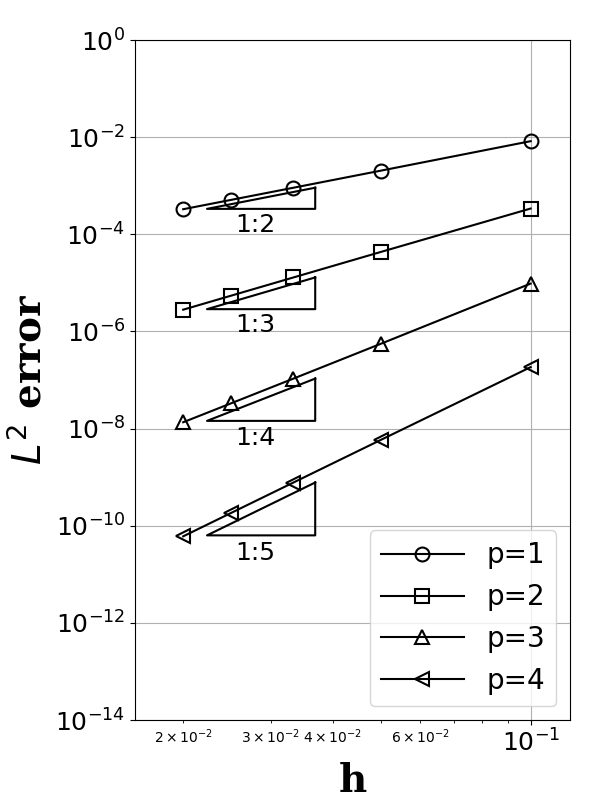
\includegraphics[width=1.0\linewidth]{figures/primal_soln_accuracy.png}
    \subcaption{Primal solution error}
    \label{fig:soln_accuracy}
  \end{subfigure}
  \begin{subfigure}{0.325\textwidth}
    \centering
    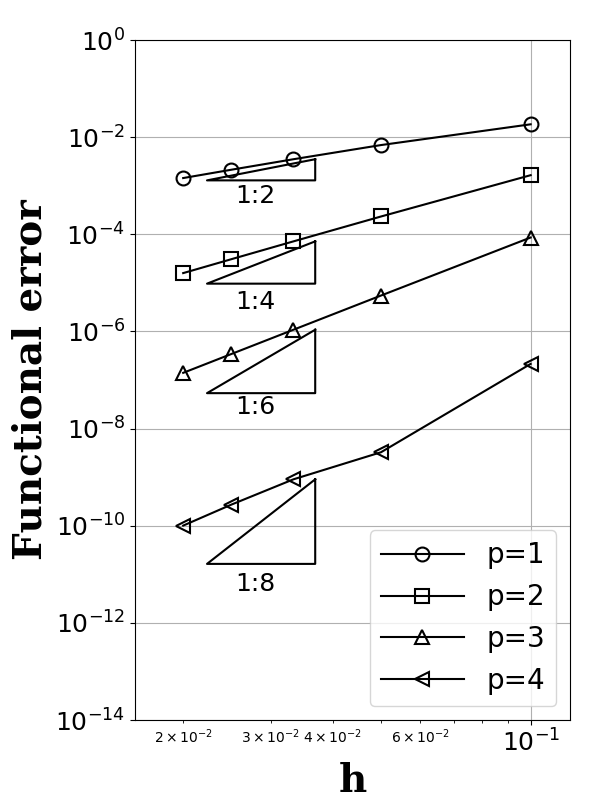
\includegraphics[width=1.0\linewidth]{figures/beta1.png}
    \subcaption{Error of $\fnc{J}$, ill-posed adjoint}
    \label{fig:func_ill}
  \end{subfigure}
  \begin{subfigure}{0.325\textwidth}
    \centering
    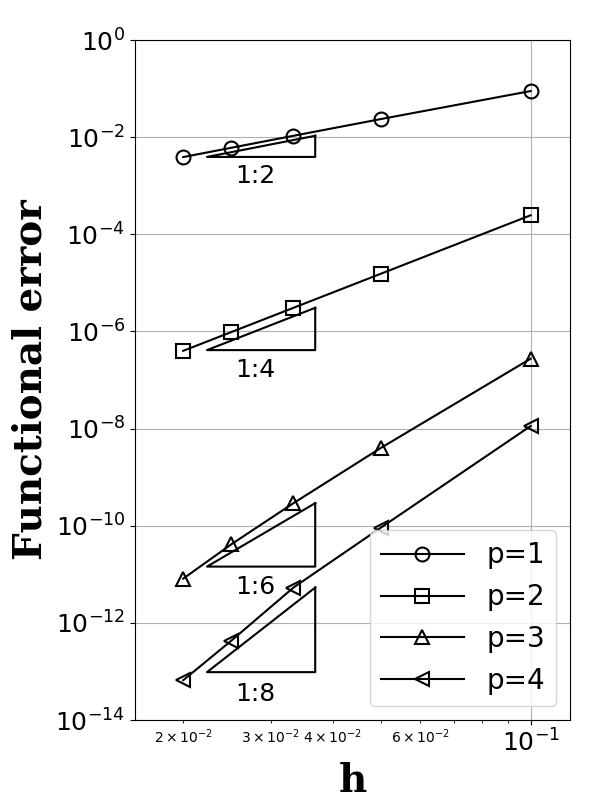
\includegraphics[width=1.0\linewidth]{figures/beta2.png}
    \subcaption{Error of $\fnc{J}$, well-posed adjoint}
    \label{fig:func_well}
  \end{subfigure}
  \caption{Convergence study}
   \label{fig:convergence} 
\end{figure}

\begin{figure}[!htbp]
	\centering
	\begin{subfigure}{0.45\textwidth}
		\centering
		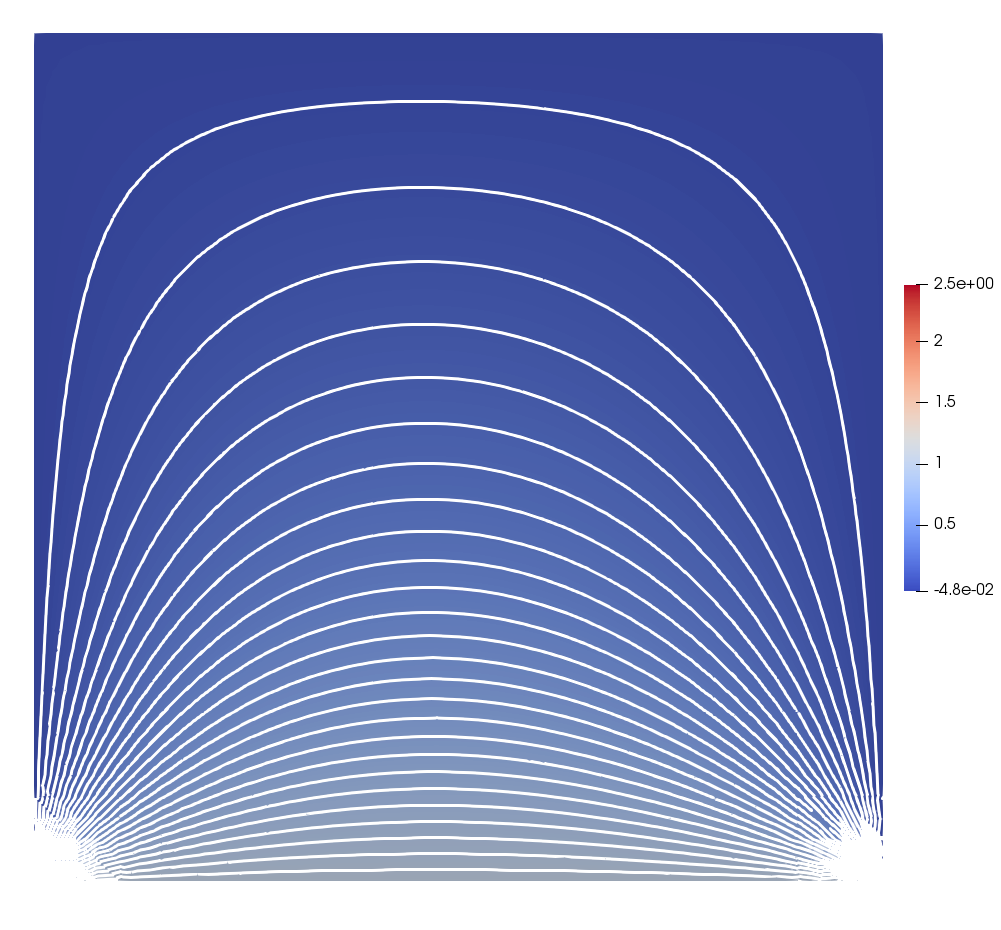
\includegraphics[width=1.0\linewidth]{figures/adj_soln_beta1.png}
		\subcaption{Ill-posed adjoint $\beta=1$}
		\label{fig:adjsln_beta1}
	\end{subfigure}
	\begin{subfigure}{0.45\textwidth}
		\centering
		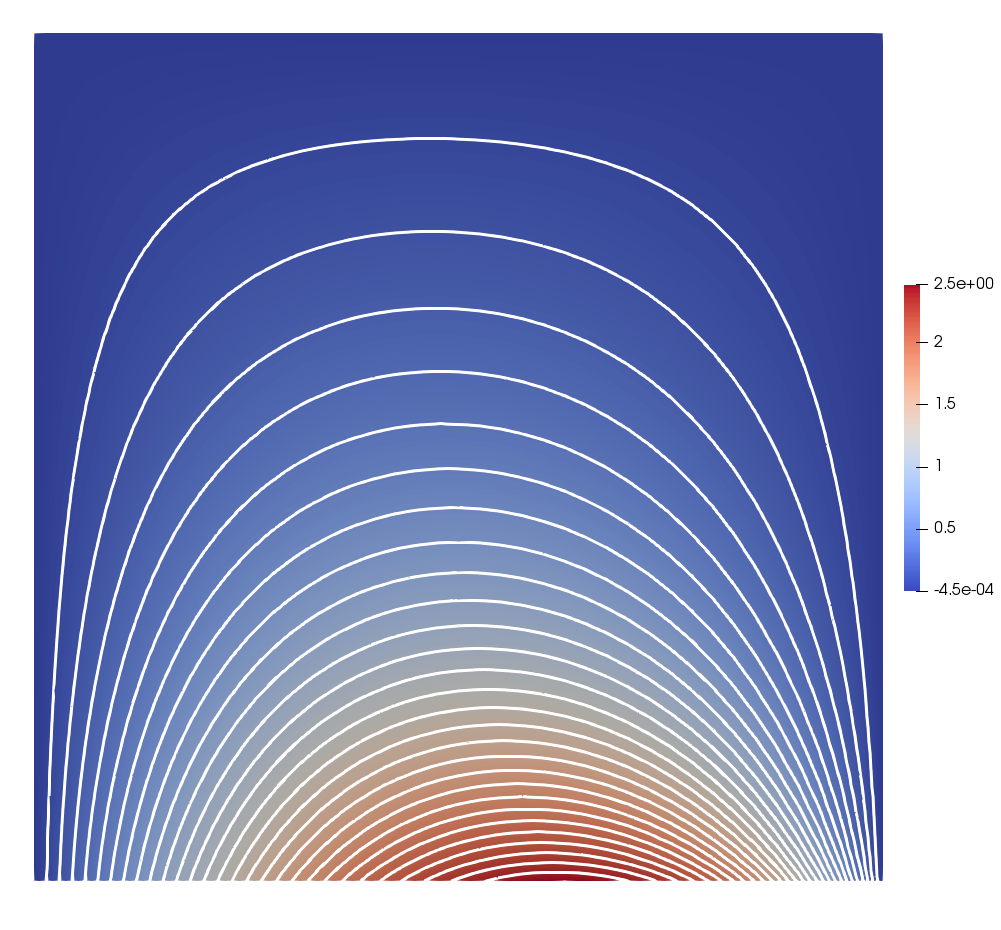
\includegraphics[width=1.0\linewidth]{figures/adj_soln_beta2.png}
		\subcaption{Well-posed adjoint with $\beta=\frac{\pi^2(e^2-1)(e-e^x)}{(e-1)^2}$}
		\label{fig:adjsln_beta2}
	\end{subfigure}
	\caption{Contours of adjoint solution} 
	\label{fig:adj_contours}
\end{figure}



\bibliographystyle{aiaa}
\bibliography{reference}
\end{document}

